\documentclass[11pt,oneside]{article}    %use"amsart"insteadof"article"forAMSLaTeXformat
\usepackage{geometry}        %Seegeometry.pdftolearnthelayoutoptions.Therearelots.
\geometry{letterpaper}        %...ora4paperora5paperor...
%\geometry{landscape}        %Activateforforrotatedpagegeometry
%\usepackage[parfill]{parskip}        %Activatetobeginparagraphswithanemptylineratherthananindent
\usepackage{graphicx}                %Usepdf,png,jpg,orepsßwithpdflatex;useepsinDVImode
                                %TeXwillautomaticallyconverteps-->pdfinpdflatex        
\usepackage{amssymb}
\usepackage[colorlinks]{hyperref}

%----macros begin---------------------------------------------------------------
\usepackage{color}
\usepackage{amsthm}

\def\conv{\mbox{\textrm{conv}\,}}
\def\aff{\mbox{\textrm{aff}\,}}
\def\E{\mathbb{E}}
\def\R{\mathbb{R}}
\def\Z{\mathbb{Z}}
\def\tex{\TeX}
\def\latex{\LaTeX}
\def\v#1{{\bf #1}}
\def\p#1{{\bf #1}}
\def\T#1{{\bf #1}}

\def\vet#1{{\left(\begin{array}{cccccccccccccccccccc}#1\end{array}\right)}}
\def\mat#1{{\left(\begin{array}{cccccccccccccccccccc}#1\end{array}\right)}}

\def\lin{\mbox{\rm lin}\,}
\def\aff{\mbox{\rm aff}\,}
\def\pos{\mbox{\rm pos}\,}
\def\cone{\mbox{\rm cone}\,}
\def\conv{\mbox{\rm conv}\,}
\newcommand{\homog}[0]{\mbox{\rm homog}\,}
\newcommand{\relint}[0]{\mbox{\rm relint}\,}

%----macros end-----------------------------------------------------------------

\title{Structured input to HIJSON\\ Towards indoor mapping and IoT modeling
\footnote{This document is part of the \emph{Linear Algebraic Representation with CoChains} (LAR-CC) framework~\cite{cclar-proj:2013:00}. \today}
}
\author{Alberto Paoluzzi}
%\date{}                            %Activatetodisplayagivendateornodate

\begin{document}
\maketitle
%\nonstopmode

\begin{abstract}
This module aims to prototype the process of entering geometric data representing a complex building, to provide them explicit semantic and a hierarchical model. The generated LAR structures~\cite{Dicarlo:2014:TNL:2543138.2543294,paodcvjcadanda2015} are finally output to HIJSON format, an experimental data format extending GEOJSON for applications of indoor mapping and the Internet-of-Things. In HIJSON  a strongly simplied building model, yet sufficient for useful purposes, accomodates the knowledge concerning the use models of the building and the set of interior devices and their connection. 
\end{abstract}

\tableofcontents

%===============================================================================
\section{Introduction}
%===============================================================================

%===============================================================================
\section{Implementation}
%===============================================================================

\subsection{Input of geometry from external drawings}
%///////////////////////////////////////////////////////////////////////////////

\paragraph{File input and computation of cellular complex}
The modeling process starts with the input of a \texttt{.svg} file, the W3C standard for 2D vector graphics on the web.
The file must only contain (by now) \texttt{<rect>} and \texttt{<line>} graphics primitives.
The geometric data generate the partition of the plane induced by an arrangment of intersecting lines.
The arrangement of (fragmented) lines is finally transformed into a 2D \emph{LAR model}, made by the triple \texttt{V,FV,EV} of vertices, faces and edges.
We notice the the LAR input is normalized by the \texttt{larFromLines} function: all vertices in \texttt{V} are transformed in the standard plane interval $[0,1]^2$.

%-------------------------------------------------------------------------------
@D SVG file input and computation of cellular complex
@{""" File input and computation of cellular complex """
def svg2lar(filename):
    lines = svg2lines(filename)
    larModel = larFromLines(lines)
    V,FV,EV = larModel
    return larModel
    
if __name__=="__main__":
    filename = "test/py/inters/plan.svg"
    larModel = svg2lar(filename)
    V,FV,EV = larModel
    FV[2] += FV[71]      # for now :o)
@}
%-------------------------------------------------------------------------------


\subsection{Emulation of interactive graphics input}
%///////////////////////////////////////////////////////////////////////////////

In this section two functions are given to emulate two graphics input primitives, respectively.

\paragraph{Emulation of input from ``selection box''}
The function accepts as input the LAR model \texttt{V,FV,EV} and a \texttt{queryBox} given in normalized coordinates. It returns \texttt{vertexSubset $\subseteq$ V, faceSubset $\subseteq$ FV, edgeSubset $\subseteq$ EV}.

%-------------------------------------------------------------------------------
@D Emulation of input from ``selection box''
@{""" Emulation of input from ``selection box'' over a LAR normalized representation """
from scipy import spatial
from bool import crossRelation,pointInPolygonClassification

def subComplexInBox(V,FV,EV,queryBox):
    (xmin,ymin),(xmax,ymax) = queryBox
    if xmin > xmax: xmin,xmax = xmax,xmin
    if ymin > ymax: ymin,ymax = ymax,ymin
    vdict = dict([(vcode(vert),k) for k,vert in enumerate(V)])
    vertexSubset = [vdict[vcode((x,y))] for x,y in V if xmin<=x<=xmax and ymin<=y<=ymax]
    edgeSubset = [e for e,edge in enumerate(EV) if all([v in vertexSubset  for v in edge])]    
    faceSubset = [f for f,face in enumerate(FV) if all([v in vertexSubset  for v in face])]
    return vertexSubset,faceSubset,edgeSubset

if __name__=="__main__":
    selectBox = ((0.45, 0.45), (0.65, 0.75))
    vertexSubset,faceSubset,edgeSubset = subComplexInBox(V,FV,EV,selectBox)
    VIEW(EXPLODE(1.2,1.2,1.2)(MKPOLS((V,[EV[e] for e in edgeSubset])) + [
    	COLOR(RED)(MK(selectBox[0])),  COLOR(RED)(MK(selectBox[1]))]))
    VIEW(EXPLODE(1.2,1.2,1.2)(MKPOLS((V,[FV[f] for f in faceSubset])) + [
    	COLOR(RED)(MK(selectBox[0])),  COLOR(RED)(MK(selectBox[1]))]))
@}
%-------------------------------------------------------------------------------

\paragraph{Emulation of  ``pick'' input over a LAR normalized representation}
The function accepts as input the LAR model \texttt{V,FV,EV}, the incidence relation \texttt{FE}, that provides for each face the list of incident edges, and a \texttt{queryPoint} given in normalized coordinates. It returns \texttt{vertexSubset $\subseteq$ V, faceSubset $\subseteq$ FV, edgeSubset $\subseteq$ EV}.

%-------------------------------------------------------------------------------
@D Emulation of ``pick'' input 
@{""" Emulation of  ``pick'' input over a LAR normalized representation """
def subComplexAroundPoint(V,FV,EV,FE,queryPoint):
    tree = spatial.cKDTree(V)
    pts = np.array([queryPoint])
    dist,closestVertex = tree.query(pts)
    VF = invertRelation(FV)
    closestFaces = VF[closestVertex]
    for face in closestFaces:
        faceEdges = [EV[e] for e in FE[face]]
        if pointInPolygonClassification(queryPoint, (V,faceEdges)) == "p_in":
            break
    vertexSubset = FV[face]
    edgeSubset = [EV[e] for e in FE[face]]
    faceSubset = [face]
    return vertexSubset,faceSubset,edgeSubset

if __name__=="__main__":
    FE = crossRelation(FV,EV)
    queryPoint = (0.6,0.58)
    vertexSubset,faceSubset,edgeSubset = subComplexAroundPoint(V,FV,EV,FE,queryPoint)
    VIEW(EXPLODE(1.2,1.2,1.2)(MKPOLS((V,[EV[e] for e in FE[faceSubset[0]]])) + [
        COLOR(RED)(MK(queryPoint))] ))
@}
%-------------------------------------------------------------------------------



\paragraph{From LAR chain to colored HPCs}
The function \texttt{cells2hpcs} is used to assign a given \texttt{k} color to the cells of a chain (cell subset) of a LAR model \texttt{V,FV}. The function returns a list of HPC (colored) objects.
%-------------------------------------------------------------------------------
@D From LAR chain to colored HPCs
@{""" From LAR chain to colored HPCs """
def cells2hpcs(V,FV,cells,k): 
    colors = [RED,GREEN,BLUE,CYAN,MAGENTA,YELLOW,WHITE,PURPLE,BROWN]
    return AA(COLOR(colors[k]))(MKPOLS((V,[FV[f] for f in cells])))
@}
%-------------------------------------------------------------------------------


\subsection{Structural operations}
%///////////////////////////////////////////////////////////////////////////////

\paragraph{From 2D chains to boundary chains}
%-------------------------------------------------------------------------------
@D From 2D chains to boundary chains
@{""" From 2D chains to boundary chains """
def chain2BoundaryChain(FV,EV):
    csrBoundaryMat = boundary(FV,EV)
    nedges,nfaces = csrBoundaryMat.shape   
    def chain2BoundaryChain0(chain):
        row = np.array(chain)
        col = np.array([0 for k in range(len(chain))])
        data = np.array([1 for k in range(len(chain))])
        csrFaceVect = scipy.sparse.coo_matrix((data, (row, col)), shape=(nfaces,1)).tocsr()
        csrEdgeVect = csrBoundaryMat*csrFaceVect
        boundaryChain = [h for h,val in 
            zip(csrEdgeVect.tocoo().row, csrEdgeVect.tocoo().data) if val%2 != 0]
        return boundaryChain
    return chain2BoundaryChain0
@}
%-------------------------------------------------------------------------------

\paragraph{From chains to structures}
%-------------------------------------------------------------------------------
@D From chains to structures
@{""" From chains to structures """
def chain2structs(V,FV,EV,FE):
    def chain2structs0(args): 
        if args == ([],[],[]): return
        chain,chainName,classtype = args
        struct = []
        for cell in chain:
            vs = [V[v] for v in FV[cell]]
            vdict = dict([[vcode(vert),k] for k,vert in enumerate(vs)])
            facetEdges = [[V[v] for v in EV[e]] for e in FE[cell]]
            ev = [(vdict[vcode(v1)], vdict[vcode(v2)]) for v1,v2 in facetEdges]
            fv = [range(len(vs))]
            shape = vs,fv,ev
            struct += [ Struct([ shape ], name=None, category="room" ) ]
        out = Struct( struct, name=chainName, category=classtype )
        return out
    return chain2structs0
@}
%-------------------------------------------------------------------------------




\paragraph{From Struct object to LAR boundary model}
%-------------------------------------------------------------------------------
@D From Struct object to LAR boundary model
@{""" From Struct object to LAR boundary model """
def structBoundaryModel(struct):
    V,FV,EV = struct2lar(struct)
    edgeBoundary = boundaryCells(FV,EV)
    cycles = boundaryCycles(edgeBoundary,EV)
    edges = [signedEdge for cycle in cycles for signedEdge in cycle]
    orientedBoundary = [ AA(SIGN)(edges), AA(ABS)(edges)]
    cells = [EV[e] if sign==1 else REVERSE(EV[e]) for (sign,e) in zip(*orientedBoundary)]
    if cells[0][0]==cells[1][0]: REVERSE(cells[0])  # bug badly patched! ... TODO better
    return V,cells
@}
%-------------------------------------------------------------------------------
    



\paragraph{From LAR oriented boundary model to polylines}
%-------------------------------------------------------------------------------
@D From LAR boundary model to polylines
@{""" From LAR oriented boundary model to polylines """
def boundaryModel2polylines(model):
    V,EV = model
    polylines = []
    succDict = dict(EV)
    visited = [False for k in range(len(V))]
    nonVisited = [k for k in succDict.keys() if not visited[k]]
    while nonVisited != []:
        first = nonVisited[0]; v = first; polyline = []
        while visited[v] == False:
            visited[v] = True; 
            polyline += V[v], 
            v = succDict[v]
        polyline += [V[first]]
        polylines += [polyline]
        nonVisited = [k for k in succDict.keys() if not visited[k]]
    return polylines
@}
%-------------------------------------------------------------------------------


\paragraph{From structures to boundary polylines}
%-------------------------------------------------------------------------------
@D From structures to boundary polylines
@{""" From structures to boundary polylines """
def boundaryPolylines(struct):
    V,boundaryEdges = structBoundaryModel(struct)
    polylines = boundaryModel2polylines((V,boundaryEdges))
    return polylines
@}
%-------------------------------------------------------------------------------





%===============================================================================
\section{Exporting the library}
%===============================================================================


%-------------------------------------------------------------------------------
@O lib/py/hijson.py
@{""" Module for Structured input to HIJSON """
from pyplasm import *
""" import modules from larcc/lib """
import sys
sys.path.insert(0, 'lib/py/')
from inters import *
from iot3d import *
from larcc import *
from bool import *
from copy import copy
DEBUG = False

@< SVG file input and computation of cellular complex @>
@< Emulation of input from ``selection box'' @>
@< Emulation of ``pick'' input @>
@< From LAR chain to colored HPCs @>
@< From 2D chains to boundary chains @>
@< From chains to structures @>
@< From Struct object to LAR boundary model @>
@< From LAR boundary model to polylines @>
@< From structures to boundary polylines @>
@}
%-------------------------------------------------------------------------------

%===============================================================================
\section{Test examples}
%===============================================================================


\subsection{Example of a complex building model: part definition}
%///////////////////////////////////////////////////////////////////////////////


\begin{figure}[htbp] %  figure placement: here, top, bottom, or page
   \centering
   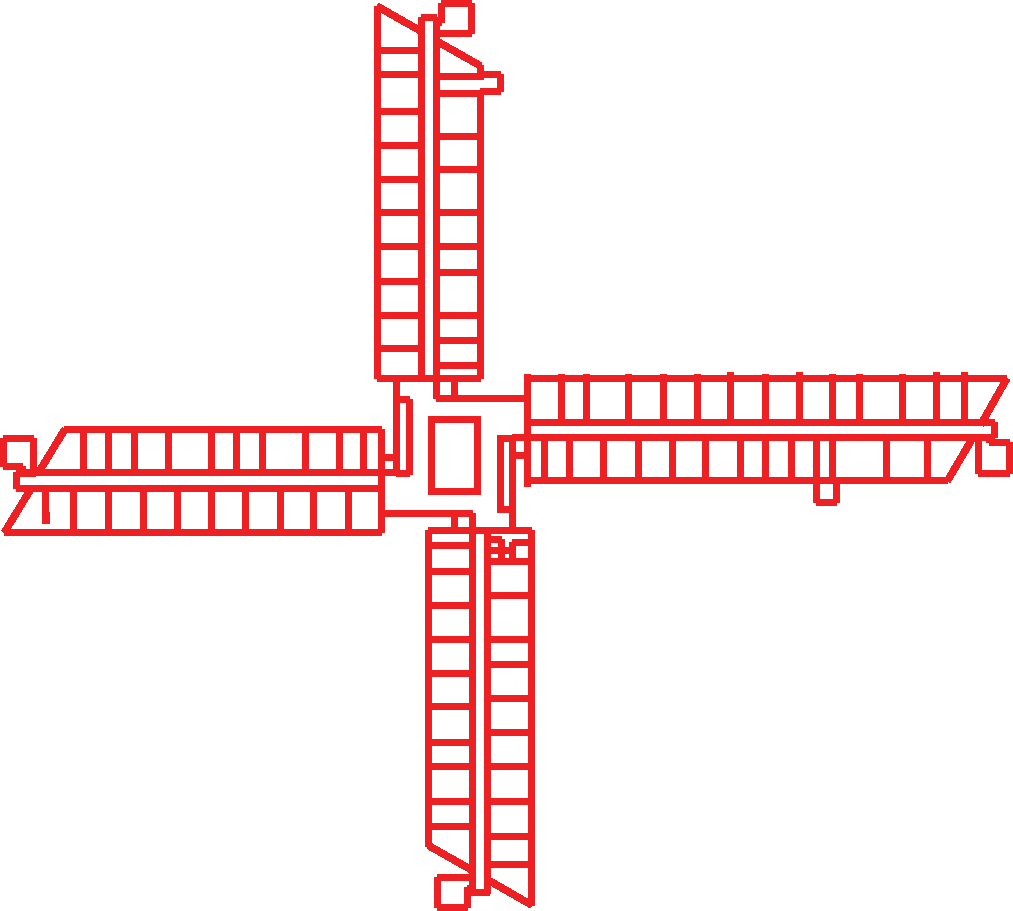
\includegraphics[width=0.55\linewidth]{images/croce} \hfill
   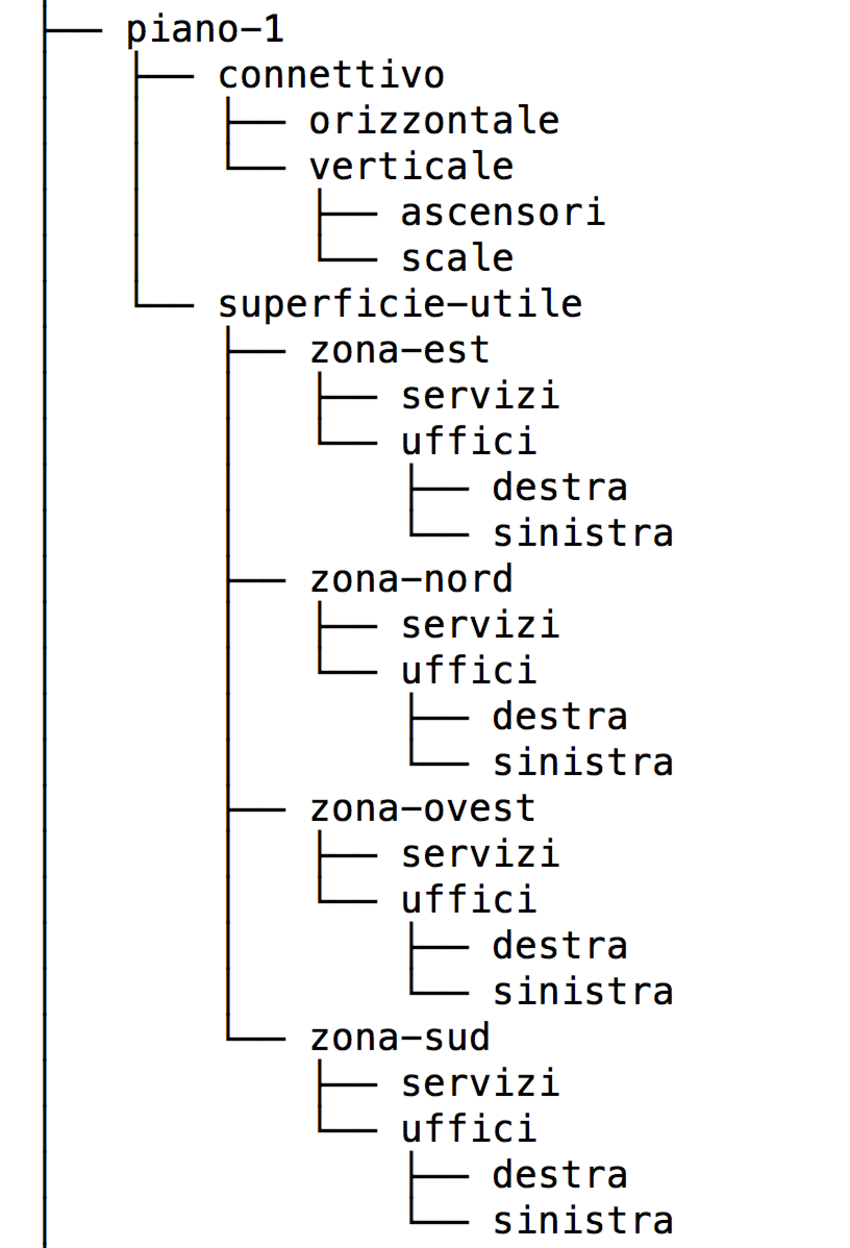
\includegraphics[width=0.35\linewidth]{images/croce2} 
   \caption{The input SVG drawing of the typical floor layout.}
   \label{fig:example}
\end{figure}


\paragraph{Visualization of cell numbering in a 2D complex}
%-------------------------------------------------------------------------------
@D Visualization of cell numbering in a 2D complex
@{""" Visualization of cell numbering in a 2D complex """
VV = AA(LIST)(range(len(V)))
submodel = STRUCT(MKPOLS((V,EV)))
VIEW(larModelNumbering(1,1,1)(V,[VV,EV,FV[:-1]],submodel,0.025))
@}
%-------------------------------------------------------------------------------


\paragraph{Ala nord (HPCs)}
%-------------------------------------------------------------------------------
@D Ala nord
@{FE = crossRelation(FV,EV)
chainsToStruct = chain2structs(V,FV,EV,FE)

""" Ala nord """
boxes = [0 for k in range(64)]
point = [0 for k in range(64)]
boxes[0] = [[0.431, 0.607], [0.474, 0.91]] #[V[k] for k in [39,208]]
boxes[1] = [[0.416, 0.657], [0.372, 0.953]] #[V[k] for k in [162,39]]
boxes[2] = [[0.416, 0.627], [0.431, 0.986]] #[V[k] for k in [206,247]]
boxes[3] = [[0.431, 0.607], [0.448, 0.627]] #[V[k] for k in [39,7]]
boxes[4] = [[0.431, 0.91], [0.494, 0.929]]  #[V[k] for k in [213,234]]
boxes[5] = [[0.431, 0.97], [0.466, 1.0]] #[V[k] for k in [58,88]]
boxes[27] = [[0.416, 0.627], [0.372, 0.657]] #[V[k] for k in [110,82]]

point[0] = [0.394, 0.9625] #CCOMB([V[k] for k in [190,197]])
point[1] = [0.4525, 0.9325] #CCOMB([V[k] for k in [166,159]])

piano1_superficieUtile_zonaNord_uffici_destra = subComplexInBox(V,FV,EV,boxes[0])[1]
piano1_superficieUtile_zonaNord_uffici_sinistra = subComplexInBox(V,FV,EV,boxes[1])[1]
piano1_connettivo_orizzontale_zonaNord = subComplexInBox(V,FV,EV,boxes[2])[1]
piano1_connettivo_verticale_zonaNord_ascensore = subComplexInBox(V,FV,EV,boxes[3])[1]
piano1_connettivo_verticale_zonaNord_ascensore += subComplexInBox(V,FV,EV,boxes[4])[1]
piano1_connettivo_verticale_zonaNord_scale = subComplexInBox(V,FV,EV,boxes[5])[1]
piano1_superficieUtile_zonaNord_servizi = subComplexAroundPoint(V,FV,EV,FE,point[0])[1]
piano1_superficieUtile_zonaNord_servizi += subComplexAroundPoint(V,FV,EV,FE,point[1])[1]
piano1_superficieUtile_zonaNord_servizi += subComplexInBox(V,FV,EV,boxes[27])[1]

piano1N = [piano1_superficieUtile_zonaNord_uffici_destra, piano1_superficieUtile_zonaNord_uffici_sinistra, piano1_connettivo_orizzontale_zonaNord, piano1_connettivo_verticale_zonaNord_ascensore, piano1_connettivo_verticale_zonaNord_scale, piano1_superficieUtile_zonaNord_servizi]
@}
%-------------------------------------------------------------------------------

%-------------------------------------------------------------------------------
@D Ala nord
@{""" Ala nord """
piano1N_nomi = ["piano1_superficieUtile_zonaNord_uffici_destra", "piano1_superficieUtile_zonaNord_uffici_sinistra", "piano1_connettivo_orizzontale_zonaNord", "piano1_connettivo_verticale_zonaNord_ascensore", "piano1_connettivo_verticale_zonaNord_scale", "piano1_superficieUtile_zonaNord_servizi"]
piano1N_categorie = ["uffici","uffici","corridoi","ascensori","scale","servizi"]
p1N = zip(piano1N,piano1N_nomi,piano1N_categorie)
piano1_zonaNord = Struct(AA(chainsToStruct)(p1N),"piano1_zonaNord","ala")
VIEW(SKEL_1(STRUCT(MKPOLS(struct2lar(piano1_zonaNord)))))
    
nord = CAT([cells2hpcs(V,FV,chain,k) for k,chain in enumerate(piano1N)])
VIEW(EXPLODE(1.2,1.2,1.2)(nord))
@}
%-------------------------------------------------------------------------------


\paragraph{Ala est (HPCs)}
%-------------------------------------------------------------------------------
@D Ala est
@{""" Ala est """
boxes[6] = [[0.019, 0.533], [0.376, 0.577]] #[V[k] for k in [241,29]]
boxes[7] = [[0.07, 0.474], [0.343, 0.518]] #[V[k] for k in [264,148]]
boxes[8] = [[0.013, 0.518], [0.376, 0.533]] #[V[k] for k in [22,63]]
boxes[9] = [[0.376, 0.533], [0.39, 0.549]] #[V[k] for k in [63,92]]
boxes[10] = [[0.001, 0.474], [0.07, 0.518]] #[V[k] for k in [263,265]]
boxes[11] = [[0.343, 0.474], [0.376, 0.518]] #[V[k] for k in [84,149]]

point[2] = [0.015, 0.5535] #CCOMB([V[k] for k in [228,14]])

piano1_superficieUtile_zonaEst_uffici_destra = subComplexInBox(V,FV,EV,boxes[6])[1]
piano1_superficieUtile_zonaEst_uffici_sinistra = subComplexInBox(V,FV,EV,boxes[7])[1]
piano1_connettivo_orizzontale_zonaEst = subComplexInBox(V,FV,EV,boxes[8])[1]
piano1_connettivo_verticale_zonaEst_ascensore = subComplexInBox(V,FV,EV,boxes[9])[1]
piano1_connettivo_verticale_zonaEst_scale = subComplexAroundPoint(V,FV,EV,FE,point[2])[1]
piano1_superficieUtile_zonaEst_servizi = subComplexInBox(V,FV,EV,boxes[10])[1]
piano1_superficieUtile_zonaEst_servizi += subComplexInBox(V,FV,EV,boxes[11])[1]

piano1E = [piano1_superficieUtile_zonaEst_uffici_destra, piano1_superficieUtile_zonaEst_uffici_sinistra, piano1_connettivo_orizzontale_zonaEst, piano1_connettivo_verticale_zonaEst_ascensore, piano1_connettivo_verticale_zonaEst_scale, piano1_superficieUtile_zonaEst_servizi]
@}
%-------------------------------------------------------------------------------
%-------------------------------------------------------------------------------
@D Ala est
@{""" Ala est """
piano1E_nomi = ["piano1_superficieUtile_zonaEst_uffici_destra", "piano1_superficieUtile_zonaEst_uffici_sinistra", "piano1_connettivo_orizzontale_zonaEst", "piano1_connettivo_verticale_zonaEst_ascensore", "piano1_connettivo_verticale_zonaEst_scale", "piano1_superficieUtile_zonaEst_servizi"]
piano1E_categorie = ["uffici","uffici","corridoi","ascensori","scale","servizi"]
p1E = zip(piano1E,piano1E_nomi, piano1E_categorie)
piano1_zonaEst = Struct(AA(chainsToStruct)(p1E), "piano1_zonaEst", "ala")
VIEW(SKEL_1(STRUCT(MKPOLS(struct2lar(piano1_zonaEst)))))

est = CAT([cells2hpcs(V,FV,chain,k) for k,chain in enumerate(piano1E)])
VIEW(EXPLODE(1.2,1.2,1.2)(est + nord))
@}
%-------------------------------------------------------------------------------


\paragraph{Ala sud (HPCs)}
%-------------------------------------------------------------------------------
@D Ala sud
@{""" Ala sud """
boxes[12] = [[0.467, 0.138], [0.423, 0.476]] #[V[k] for k in [252,47]]
boxes[13] = [[0.482, 0.145], [0.525, 0.445]] #[V[k] for k in [241,126]]
boxes[14] = [[0.482, 0.476], [0.467, 0.116]] #[V[k] for k in [254,232]]
boxes[15] = [[0.449, 0.476], [0.467, 0.493]] #[V[k] for k in [40,237]]
boxes[16] = [[0.431, 0.101], [0.467, 0.131]] #[V[k] for k in [259,2]]
boxes[17] = [[0.482, 0.445], [0.525, 0.476]] #[V[k] for k in [155,248]]
boxes[18] = [[0.525, 0.104], [0.482, 0.145]] #[V[k] for k in [111,241]]

piano1_superficieUtile_zonaSud_uffici_destra = subComplexInBox(V,FV,EV,boxes[12])[1]
piano1_superficieUtile_zonaSud_uffici_sinistra = subComplexInBox(V,FV,EV,boxes[13])[1]
piano1_connettivo_orizzontale_zonaSud = subComplexInBox(V,FV,EV,boxes[14])[1]
piano1_connettivo_verticale_zonaSud_ascensore = subComplexInBox(V,FV,EV,boxes[15])[1]
piano1_connettivo_verticale_zonaSud_scale = subComplexInBox(V,FV,EV,boxes[16])[1]
piano1_superficieUtile_zonaSud_servizi = subComplexInBox(V,FV,EV,boxes[17])[1]
piano1_superficieUtile_zonaSud_servizi += subComplexInBox(V,FV,EV,boxes[18])[1]

piano1S = [piano1_superficieUtile_zonaSud_uffici_destra, piano1_superficieUtile_zonaSud_uffici_sinistra, piano1_connettivo_orizzontale_zonaSud, piano1_connettivo_verticale_zonaSud_ascensore, piano1_connettivo_verticale_zonaSud_scale, piano1_superficieUtile_zonaSud_servizi]
@}
%-------------------------------------------------------------------------------

%-------------------------------------------------------------------------------
@D Ala sud
@{""" Ala sud """
piano1S_nomi = ["piano1_superficieUtile_zonaSud_uffici_destra", "piano1_superficieUtile_zonaSud_uffici_sinistra", "piano1_connettivo_orizzontale_zonaSud", "piano1_connettivo_verticale_zonaSud_ascensore", "piano1_connettivo_verticale_zonaSud_scale", "piano1_superficieUtile_zonaSud_servizi"]
piano1S_categorie = ["uffici","uffici","corridoi","ascensori","scale","servizi"]
p1S = zip(piano1S,piano1S_nomi, piano1S_categorie)
piano1_zonaSud = Struct(AA(chainsToStruct)(p1S), "piano1_zonaSud", "ala")
VIEW(SKEL_1(STRUCT(MKPOLS(struct2lar(piano1_zonaSud)))))
    
sud = CAT([cells2hpcs(V,FV,chain,k) for k,chain in enumerate(piano1S)])
VIEW(EXPLODE(1.2,1.2,1.2)(est + nord + sud))
@}
%-------------------------------------------------------------------------------


\paragraph{Ala ovest (HPCs)}
%-------------------------------------------------------------------------------
@D Ala ovest
@{""" Ala ovest """
boxes[19] = [[0.521, 0.526], [0.963, 0.568]] #[V[k] for k in [169,202]]
boxes[20] = [[0.555, 0.584], [0.955, 0.627]] #[V[k] for k in [12,23]]
boxes[21] = [[0.521, 0.568], [0.985, 0.584]] #[V[k] for k in [209,204]]
boxes[22] = [[0.506, 0.551], [0.521, 0.568]] #[V[k] for k in [89,209]]
boxes[23] = [[0.808, 0.504], [0.828, 0.526]] #[V[k] for k in [270,77]]
boxes[24] = [[0.955, 0.584], [0.997, 0.627]] #[V[k] for k in [220,24]]
boxes[25] = [[0.521, 0.584], [0.555, 0.627]] #[V[k] for k in [11,144]]
boxes[26] = [[1.0, 0.533], [0.97, 0.568]] #[V[k] for k in [233,201]]

piano1_superficieUtile_zonaOvest_uffici_destra = subComplexInBox(V,FV,EV,boxes[19])[1]
piano1_superficieUtile_zonaOvest_uffici_sinistra = subComplexInBox(V,FV,EV,boxes[20])[1]
piano1_connettivo_orizzontale_zonaOvest = subComplexInBox(V,FV,EV,boxes[21])[1]
piano1_connettivo_verticale_zonaOvest_ascensore = subComplexInBox(V,FV,EV,boxes[22])[1]
piano1_connettivo_verticale_zonaOvest_ascensore += subComplexInBox(V,FV,EV,boxes[23])[1]
piano1_superficieUtile_zonaOvest_servizi = subComplexInBox(V,FV,EV,boxes[24])[1]
piano1_superficieUtile_zonaOvest_servizi += subComplexInBox(V,FV,EV,boxes[25])[1]
piano1_connettivo_verticale_zonaOvest_scale = subComplexInBox(V,FV,EV,boxes[26])[1]

piano1O = [piano1_superficieUtile_zonaOvest_uffici_destra, piano1_superficieUtile_zonaOvest_uffici_sinistra, piano1_connettivo_orizzontale_zonaOvest, piano1_connettivo_verticale_zonaOvest_ascensore, piano1_connettivo_verticale_zonaOvest_scale, piano1_superficieUtile_zonaOvest_servizi]
@}
%-------------------------------------------------------------------------------

%-------------------------------------------------------------------------------
@D Ala ovest
@{""" Ala ovest """
piano1O_nomi = ["piano1_superficieUtile_zonaOvest_uffici_destra", "piano1_superficieUtile_zonaOvest_uffici_sinistra", "piano1_connettivo_orizzontale_zonaOvest", "piano1_connettivo_verticale_zonaOvest_ascensore", "piano1_connettivo_verticale_zonaOvest_scale", "piano1_superficieUtile_zonaOvest_servizi"]
piano1O_categorie = ["uffici","uffici","corridoi","ascensori","scale","servizi"]
p1O = zip(piano1O,piano1O_nomi, piano1O_categorie)
piano1_zonaOvest = Struct(AA(chainsToStruct)(p1O), "piano1_zonaOvest", "ala")
VIEW(SKEL_1(STRUCT(MKPOLS(struct2lar(piano1_zonaOvest)))))
    
ovest = CAT([cells2hpcs(V,FV,chain,k) for k,chain in enumerate(piano1O)])
VIEW(EXPLODE(1.2,1.2,1.2)(est + nord + sud + ovest))
@}
%-------------------------------------------------------------------------------


\paragraph{Centro stella (HPCs)}
%-------------------------------------------------------------------------------
@D Centro stella
@{""" Centro stella """
piano1_connettivo_orizzontale_centroStella = [2]
piano1_connettivo_verticale_centroStella_scale = [15,26]

piano1C = [[],[],piano1_connettivo_orizzontale_centroStella,[], piano1_connettivo_verticale_centroStella_scale]
centro = CAT([cells2hpcs(V,FV,chain,k) for k,chain in enumerate(piano1C)])
@}
%-------------------------------------------------------------------------------

%-------------------------------------------------------------------------------
@D Centro stella
@{""" Centro stella """
piano1C_nomi = [[],[],"piano1_connettivo_orizzontale_centroStella", [], "piano1_connettivo_verticale_centroStella_scale"]
piano1C_categorie = [[],[],"corridoi",[], "ascensori"]
p1C = zip(piano1C,piano1C_nomi, piano1C_categorie)
piano1_centroStella = Struct(AA(chainsToStruct)(p1C), "piano1_centroStella", "centro")
VIEW(SKEL_1(STRUCT(MKPOLS(struct2lar(piano1_centroStella)))))

VIEW(EXPLODE(1.2,1.2,1.2)(est + nord + sud + ovest + centro))
VIEW(STRUCT(est + nord + sud + ovest + centro))
@}
%-------------------------------------------------------------------------------


\subsection{Example of a complex building model: integration}
%///////////////////////////////////////////////////////////////////////////////

\paragraph{Assembly of parts (HPCs)}
%-------------------------------------------------------------------------------
@D Assemblaggio
@{""" Assemblaggio """
p1 = p1N + p1S + p1E + p1O + p1C

piano1_nomi = ["piano1_zonaNord", "piano1_zonaEst", "piano1_zonaSud", "piano1_zonaOvest", "piano1_centroStella"]
piano1_categorie = ["ala","ala","ala","ala","centro"]
piano1 = Struct(AA(chainsToStruct)(p1), "piano1", "piano")

VIEW(SKEL_1(STRUCT(MKPOLS(struct2lar(piano1)))))

V,boundaryEdges = structBoundaryModel(piano1)
drawing = mkSignedEdges((V,boundaryEdges))
VIEW(drawing)
        
polylines = boundaryModel2polylines((V,boundaryEdges))
VIEW(STRUCT(AA(POLYLINE)(polylines)))
    
print boundaryPolylines(piano1)
@}
%-------------------------------------------------------------------------------


\paragraph{Assembling floor layout generation}
%-------------------------------------------------------------------------------
@D Assembling floor layout generation
@{""" Assembling floor layout generation """
@< Visualization of cell numbering in a 2D complex @>
@< Ala nord @>
@< Ala est @>
@< Ala sud @>
@< Ala ovest @>
@< Centro stella @>
@< Assemblaggio @>
@}
%-------------------------------------------------------------------------------



%-------------------------------------------------------------------------------
@D Tower example initialization
@{""" make the model of a layout floor """
""" import modules from larcc/lib """
import sys
sys.path.insert(0, 'lib/py/')
from hijson import *

filename = "test/py/inters/plan.svg"
larModel = svg2lar(filename)
V,FV,EV = larModel
FV[2] += FV[71]      # for now :o)
@}
%-------------------------------------------------------------------------------

%-------------------------------------------------------------------------------
@O test/py/hijson/test01.py
@{""" make the model of a layout floor """
@< Tower example initialization @>
@< Assembling floor layout generation @>
@}
%-------------------------------------------------------------------------------


%-------------------------------------------------------------------------------
@D Exploring the tower generation
@{""" Exploring the floor layout generation """
@< Assembling floor layout generation @>

piano = Struct([piano1_zonaNord,piano1_zonaEst,piano1_zonaSud,piano1_zonaOvest, piano1_centroStella], "pianoTipo","piano")
print "\npiano =",piano
print "piano.dim =",piano.dim

Vp,FVp,EVp = struct2lar(piano)
VIEW(EXPLODE(1.2,1.2,1.2)(MKPOLS((Vp,EVp))))

piano3D = embedStruct(1)(piano,"3D")
print "\npiano3D =",piano3D
print "piano3D.dim =",piano3D.dim
print "piano3D.body =",piano3D.body

print "\npiano3D.body[0] =",piano3D.body[0]
print "piano3D.body[0].body =",piano3D.body[0].body
print "piano3D.body[0].body[0] =",piano3D.body[0].body[0]
print "piano3D.body[0].body[0].body =",piano3D.body[0].body[0].body
print "piano3D.body[0].body[0].body[0] =",piano3D.body[0].body[0].body[0]
print "piano3D.body[0].body[0].body[0].body =",piano3D.body[0].body[0].body[0].body
@}
%-------------------------------------------------------------------------------

%-------------------------------------------------------------------------------
@O test/py/hijson/test02.py
@{""" make the 2.5 model of a building tower """
@< Tower example initialization @>
@< Assembling floor layout generation @>
@< Exploring the tower generation @>

pianoNord3D = embedStruct(1)(piano1_zonaNord,"3D")
torreNord = Struct(6*[pianoNord3D,t(0,0,0.03)], "torreNord", "edificio2.5D")
V,FV,EV = struct2lar(torreNord)
VIEW(EXPLODE(1.2,1.2,1.2)(MKPOLS((V,EV))))
@}
%-------------------------------------------------------------------------------


\bibliographystyle{amsalpha}
\bibliography{hijson}

\end{document}
